\documentclass[12pt]{article}
\usepackage[pdftex]{graphics}
\usepackage{tikz}

\usetikzlibrary{circuits} 
\usetikzlibrary{circuits.ee} 
\usetikzlibrary{circuits.ee.IEC}
\usetikzlibrary{arrows}
\usetikzlibrary{patterns} 

\begin{document}

Super desctription of LC-circuit.

\begin{figure}[!h]
\begin{center}
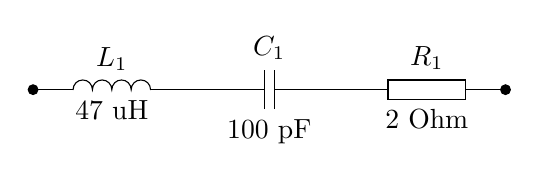
\begin{tikzpicture}[circuit ee IEC]
\node (in) at (0,0) [contact] {}; 
\node (L1) at (1,0) [inductor={info = $L_1$, info'= 47 uH}] {}; 
\node (C1) at (3,0) [capacitor={info = $C_1$, info'= 100 pF}] {};
\node (R) at (5,0) [resistor={info = $R_1$, info'= 2 Ohm}] {};
\node (out) at (6,0) [contact] {};
\draw (in) -- (L1) -- (C1) -- (R) -- (out);
\end{tikzpicture}
\end{center}
\caption{LC-contour}
\end{figure}

RC and its amplitude frequency response.

\begin{figure}[!h]
\begin{center}
\begin{tikzpicture}[circuit ee IEC]
\node (R) [resistor={info={$R$}}] at (2,2) {};
\node (p1) [contact] at (3,2) {};
\node (C) [point up,
capacitor={info={$C$}}] at (3,1) {}; 
\node (p2) [contact] at (3,0) {};
\draw [-latex] (p1) -- (5,2);
\draw [latex-] (0,2) -- (R);
\draw (R) -- (p1) -- (C) -- (p2);
\draw [latex-] (0,0) -- (p2);
\draw [-latex] (p2) -- (5,0);
\node  at (0,1) {Input};
\node  at (5,1) {Output};


\draw[xshift=60mm,-latex] (0,0) -- (4,0)
node [anchor=west]
{$\omega$};
\draw[xshift=60mm,-latex] (0,0) -- (0,3)
node [anchor=south]
{$K(\omega)$};
\draw [very
thick,xshift=60mm, y=2cm, x=1cm,
declare function={K(\w)=1/sqrt(1+\w^2);}] plot [domain=0:3, samples=10,
smooth] (\x,{K(\x)});
\end{tikzpicture}
\end{center}
\caption{Amplitude-frequency response}
\end{figure}


\begin{figure}[!ht]
\begin{center}
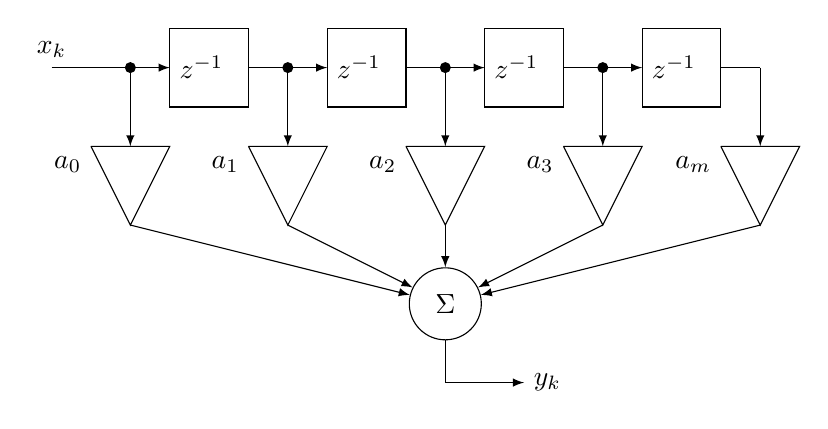
\begin{tikzpicture}
\draw (-10mm,0) node [anchor=south] {$x_k$}-- (0,0);

\node (s) at (40mm,-30mm)  [circle,draw, inner sep=2mm] {$\Sigma$};

\foreach \x / \a in {0mm/$a_0$,20mm/$a_1$,40mm/$a_2$,60mm/$a_3$}
{
\fill (\x,0) circle (0.7mm);
\draw [-latex] (\x,0)--(\x+5mm,0);
\draw (\x+5mm, -5mm)rectangle (\x+15mm,5mm);
\draw (\x+5mm,0) node [anchor=west] {$z^{-1}$};
\draw [-latex] (\x,0) -- (\x,-10mm);
\draw (\x-5mm,-10mm) node [anchor=north east] {\a} -- (\x+5mm,-10mm) --
(\x,-20mm) -- (\x-5mm,-10mm);
\draw  (\x+15mm,0)--(\x+20mm,0);
\draw [-latex] (\x,-20mm) -- (s);
}
\draw [-latex] (80mm,0) -- (80mm,-10mm);
\draw (75mm,-10mm) node [anchor=north east] {$a_m$} -- (85mm,-10mm) --
(80mm,-20mm) -- (75mm,-10mm);
\draw [-latex] (80mm,-20mm) -- (s);
\draw [-latex] (s)--(40mm,-40mm)--(50mm,-40mm) node [anchor=west] {$y_k$};
\end{tikzpicture} 
\end{center}
\caption{Finite impulse response (FIR) digital filter}
\end{figure}

\end{document}
